\chapter{Subspaces, Projection Operators, and Measurement as Entanglement}

This chapter follows Leonard Susskind's sixth lecture in the Quantum Entanglement series, curated by LazyingArt LLC. The order matters. We begin in the wake of Bell's theorem, where locality and entanglement are still pressing on the room; then we step back and rebuild the mathematics of subspaces and projection operators at an elementary level; only after that do we return to measurement, now through a finite-state version of the two-slit experiment. The payoff is the lecture's central claim: a measurement is the establishment of entanglement between a system and an apparatus, and it is exactly this recording of information that destroys interference.

\section{Opening Motivation: Entanglement, Locality, and Measurement}

The lecture does not open with a clean new topic. It begins inside the unresolved discomfort left by Bell's theorem. If one member of an entangled pair is measured, what happens on the other side? Susskind's answer is deliberately operational: nothing detectable happens there, and no usable message arrives there. One may act locally on one member of the pair, even rotate its spin with a magnetic field, and thereby change the detailed form of the two-particle state, but the distant particle remains entangled with whatever system lives on the other side.

That is already enough to shift the discussion away from the naive idea that entanglement is a relation between two little labeled particles and nothing else. If one particle falls into a black hole, the other does not cease to be entangled; rather, it is entangled with the larger system containing the black hole degrees of freedom and, later, the radiation emitted from the black hole. Susskind then replaces the black hole by a bathtub, precisely to make the point less exotic. Drop one member of an entangled pair into the tub, let it mix with everything there, and the distant particle is no longer entangled with one neatly identifiable partner; it is entangled with the state of the bathtub.

This is not only a story about persistence. It is also a story about reversibility. If interaction can create entanglement, then interaction can in principle undo it. Disentanglement is possible, but only if the systems come back into causal contact and interact again.

The room then asks the right question. Suppose two electrons are entangled and we measure them. Are they still entangled afterwards, or does the measurement kick them out? Susskind answers that the measurements do kick them out, or at least can. That answer is held in suspense for a few moments, because he immediately says what the real destination of the lecture will be: the relation among measurement, collapse of the wave packet, and entanglement. But before going there, he wants to repair the mathematics of subspaces and projection operators.

\section{Dimension, Linear Dependence, and Orthonormal Bases}

We stay, for the moment, with finite-dimensional vector spaces equipped with bras, kets, and an inner product. The first thing to make precise is dimension. Susskind does not define it by counting entries in a column vector. He defines it geometrically and abstractly: the dimension of the space is the maximum number of linearly independent vectors that can be found in it.

In symbols, a set of vectors \(|v_i\rangle\) is linearly independent if the only relation
\begin{equation}
\sum_i c_i |v_i\rangle = 0
\end{equation}
is the trivial one in which all coefficients vanish. Equivalently, no one of the vectors can be expressed as a linear combination of the others.

It is important that orthogonality and linear independence are not the same thing. In three dimensions, three non-orthogonal vectors can still be linearly independent, provided one of them cannot be built from the other two. On the other hand, in a two-dimensional plane, any third vector lying in that plane is necessarily linearly dependent on the first two.

\begin{figure}[htbp]
\centering

\includegraphics[width=0.56\textwidth]{lecture_06_figure_02.png}
\caption{Three vectors on the board. The lecture uses this sketch to distinguish linear independence from orthogonality and then to emphasize that in a plane a third vector is dependent on the first two.}
\end{figure}

\begin{figure}[htbp]
\centering
\begin{tikzpicture}[scale=1.2]
\draw[->] (0,0) -- (2.3,0);
\draw[->] (0,0) -- (2.0,2.0);
\draw[->] (0.35,0.95) -- (1.05,1.45);
\fill (0,0) circle (1.2pt);
\end{tikzpicture}
\caption{A minimal reconstruction of the board sketch. The exact coefficients relating the vectors are not fixed by the frame alone; the geometric point is that in a two-dimensional plane a third vector is not independent.}
\end{figure}

Thus, if the space is two-dimensional, the maximum number of linearly independent vectors is two. If the space is three-dimensional, it is three. More generally, if the space has dimension \(d\), then one can find \(d\) mutually orthogonal unit vectors spanning it. Those are basis vectors. They are not unique, but once a basis has been chosen, every vector in the space can be expanded in it.

\subsection{Question \& Answer: Are spatial degrees of freedom the same thing as the dimension of the state space?}

No. A particle moving in three-dimensional space has three spatial degrees of freedom in the ordinary mechanical sense, but that fact does not determine the dimension of its space of states. The state space can be vastly larger. In the finite-dimensional examples of this lecture we deliberately work with a small state space, but that is a pedagogical simplification, not a statement that the dimension of Hilbert space is the same thing as the number of spatial directions available to the particle.

\section{Basis Expansion, Dyads, and the Resolution of Identity}

Choose an orthonormal basis \(\{|n\rangle\}\), with \(n=1,\dots,d\). The blackboard now settles into its standard form:

\begin{figure}[htbp]
\centering

\includegraphics[width=0.62\textwidth]{lecture_06_figure_03.png}
\caption{Orthonormal basis and expansion of an arbitrary state.}
\end{figure}

We write
\begin{align}
\langle m|n\rangle &= \delta_{mn}, \\
|\psi\rangle &= \sum_n a_n |n\rangle.
\end{align}
Here \(\delta_{mn}\) is the Kronecker delta: it is \(1\) when \(m=n\) and \(0\) otherwise.

\paragraph{Worked derivation.} The expansion coefficients are immediately recovered by projecting onto the basis. Multiply the expansion by \(\langle m|\) from the left:
\begin{align}
\langle m|\psi\rangle
  &= \sum_n a_n \langle m|n\rangle \\
  &= \sum_n a_n \delta_{mn} \\
  &= a_m.
\end{align}
So the coefficients are not mysterious objects at all:
\begin{equation}
a_m = \langle m|\psi\rangle.
\end{equation}

Insert that result back into the expansion:
\begin{equation}
|\psi\rangle = \sum_n |n\rangle \langle n|\psi\rangle.
\end{equation}
This suggests that the object \(|n\rangle\langle n|\), and more generally \(|a\rangle\langle b|\), should be interpreted as an operator. Indeed, the dyad \(|a\rangle\langle b|\) acts on an arbitrary state by
\begin{equation}
\bigl(|a\rangle\langle b|\bigr)|\psi\rangle = \langle b|\psi\rangle\,|a\rangle.
\end{equation}
The bra extracts a complex number; the ket then supplies the direction of the resulting vector.

Now read the expansion operatorially. Since
\begin{equation}
|\psi\rangle = \left(\sum_n |n\rangle\langle n|\right)|\psi\rangle
\end{equation}
for every \(|\psi\rangle\), the sum in parentheses must be the identity operator:
\begin{equation}
\sum_n |n\rangle\langle n| = I.
\end{equation}
This is the resolution of the identity. It is the operator version of the statement that the basis spans the whole space.

Susskind briefly pauses here to note that \(I\) is a very special observable. Every vector is an eigenvector of \(I\), and every eigenvalue is \(+1\). In that sense, the identity is the projection operator onto the whole space.

\section{Properties as Subspaces and Projection Operators}

Now comes the conceptual correction on which the rest of the lecture depends. A property such as \(k=\lambda\) is not, in general, a single vector. It is a whole subspace.

Suppose \(k\) is a Hermitian observable and that
\begin{equation}
k|A\rangle = \lambda |A\rangle, \qquad
k|B\rangle = \lambda |B\rangle,
\end{equation}
with \(|A\rangle\) and \(|B\rangle\) linearly independent. Then any linear combination also has the same eigenvalue:
\begin{align}
k\bigl(\alpha|A\rangle+\beta|B\rangle\bigr)
  &= \alpha k|A\rangle + \beta k|B\rangle \\
  &= \alpha \lambda |A\rangle + \beta \lambda |B\rangle \\
  &= \lambda \bigl(\alpha|A\rangle+\beta|B\rangle\bigr).
\end{align}
So the eigenspace corresponding to \(\lambda\) is closed under addition and scalar multiplication. It is a subspace.

The lecture gives a concrete two-spin example. The states
\begin{equation}
|ud\rangle,\qquad |uu\rangle
\end{equation}
have different values of the second spin, but they agree on the first spin: the first spin is up in both cases, so both lie in the subspace with \(\sigma_3=+1\) for the first spin.

\begin{figure}[htbp]
\centering

\includegraphics[width=0.46\textwidth]{lecture_06_figure_04.png}
\caption{Two two-spin states with first spin up.}
\end{figure}

If \(\{|a\rangle\}\) is an orthonormal basis for the eigensubspace \(k=\lambda\), then the projection operator onto that subspace is
\begin{equation}
\Pi_{k=\lambda}=\sum_a |a\rangle\langle a|.
\end{equation}
The sum now runs only over a basis of the subspace, not over a basis of the whole space. If \(|\psi\rangle\) already lies in the subspace, \(\Pi_{k=\lambda}|\psi\rangle = |\psi\rangle\). If \(|\psi\rangle\) has components outside the subspace, the projector throws those away and keeps only the component inside.

That is the geometric meaning of projection, and Susskind leans on it heavily.

\begin{figure}[htbp]
\centering

\includegraphics[width=0.44\textwidth]{lecture_06_figure_06.png}
\caption{The projected state as a vector in the eigensubspace.}
\end{figure}

\begin{figure}[htbp]
\centering
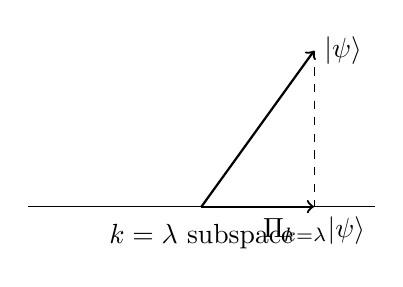
\begin{tikzpicture}[scale=1.1]
\draw (-2,0) -- (2,0);
\draw[->,thick] (0,0) -- (1.3,1.8) node[right] {$|\psi\rangle$};
\draw[dashed] (1.3,1.8) -- (1.3,0);
\draw[->,thick] (0,0) -- (1.3,0) node[below] {$\Pi_{k=\lambda}|\psi\rangle$};
\node at (0,-0.35) {$k=\lambda$ subspace};
\end{tikzpicture}
\caption{A geometric reconstruction of the lecture's point: \(\Pi_{k=\lambda}|\psi\rangle\) lies in the \(k=\lambda\) eigensubspace.}
\end{figure}

In the lecture this is not merely a picture. It is the algebraic statement that
\begin{equation}
k\bigl(\Pi_{k=\lambda}|\psi\rangle\bigr)=\lambda\,\Pi_{k=\lambda}|\psi\rangle.
\end{equation}
So the projected vector really is a vector with the property \(k=\lambda\).

\section{Probability Postulate, Compatible Properties, and the Bell Recap}

Once a property has been identified with a subspace, the probability postulate takes its cleanest form. The probability that a normalized state \(|\psi\rangle\) has the property \(k=\lambda\) is
\begin{equation}
P(k=\lambda)=\langle\psi|\Pi_{k=\lambda}|\psi\rangle.
\end{equation}

\begin{figure}[htbp]
\centering

\includegraphics[width=0.58\textwidth]{lecture_06_figure_05.png}
\caption{Projector onto the \(k=\lambda\) eigensubspace. The blackboard layout already suggests the next step: sandwich the projector between \(\langle\psi|\) and \(|\psi\rangle\).}
\end{figure}

If we insert the dyadic form of the projector, we obtain
\begin{align}
P(k=\lambda)
  &= \left\langle \psi \left| \sum_a |a\rangle\langle a| \right| \psi \right\rangle \\
  &= \sum_a \langle\psi|a\rangle \langle a|\psi\rangle \\
  &= \sum_a |\langle a|\psi\rangle|^2.
\end{align}
This is exactly the lecture's interpretation: the probability for the property is the sum of the probabilities of all the orthogonal ways the property can be realized.

For the first spin being up in a two-spin system, the relevant subspace is spanned by \(|uu\rangle\) and \(|ud\rangle\), so
\begin{equation}
\Pi_{\sigma_3=+1}=|uu\rangle\langle uu|+|ud\rangle\langle ud|.
\end{equation}
In the blackboard shorthand of the lecture, one also writes
\begin{equation}
\Pi_{\sigma_3=+1}=\frac{1+\sigma_3}{2},
\end{equation}
with the identity on the second spin understood.

Now suppose we have two compatible properties, represented by commuting projectors \(P_k\) and \(P_\ell\). The lecture's algebraic version of the logical AND statement is
\begin{equation}
\Pi_{k=\lambda \,\wedge\, \ell=\mu}=P_kP_\ell=P_\ell P_k.
\end{equation}
The reason is straightforward. \(P_k|\psi\rangle\) lies in the \(k=\lambda\) subspace. If \(P_k\) and \(P_\ell\) commute, then \(P_\ell P_k|\psi\rangle = P_k P_\ell|\psi\rangle\) lies in both subspaces at once. Therefore the probability of the simultaneous property is
\begin{equation}
P(k=\lambda,\ell=\mu)=\langle\psi|P_kP_\ell|\psi\rangle.
\end{equation}

\begin{figure}[htbp]
\centering
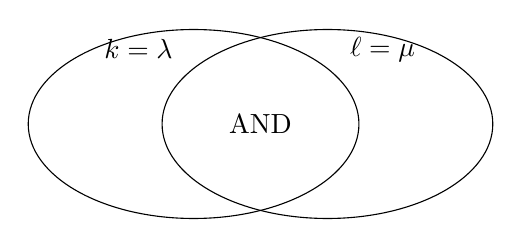
\begin{tikzpicture}[scale=1.0]
\draw (0,0) ellipse (2.1 and 1.2);
\draw (1.7,0) ellipse (2.1 and 1.2);
\node at (-0.7,0.95) {$k=\lambda$};
\node at (2.4,0.95) {$\ell=\mu$};
\node at (0.85,0) {AND};
\end{tikzpicture}
\caption{A clean reconstruction of the intersecting-subspace picture behind the AND statement for commuting projectors.}
\end{figure}

\begin{remark}
The lecture also treats the OR statement, in this same compatible-projector setting, as the sum of the projectors. We keep that claim in the limited context in which it is used here and do not need a more general formula.
\end{remark}

At this point Susskind returns to Bell's theorem. The classical inequality, written in terms of probabilities rather than counts, is
\begin{equation}
P(A\wedge \neg B)+P(B\wedge \neg C)\ge P(A\wedge \neg C).
\end{equation}
That inequality is a theorem of classical set logic, not of quantum mechanics. In the singlet state, the spins are always opposite along any common axis, so a NOT statement for the first spin can be traded for the corresponding positive statement for the second spin. The lecture then rewrites the three relevant clauses as joint properties of a two-spin system.

Suppressing identity operators on untouched factors, the elementary single-property projectors are
\begin{equation}
\frac{1+\sigma_3}{2},\qquad
\frac{1+\frac{\tau_1+\tau_3}{\sqrt2}}{2},\qquad
\frac{1+\frac{\sigma_1+\sigma_3}{\sqrt2}}{2},\qquad
\frac{1+\tau_1}{2}.
\end{equation}
Therefore the three joint projectors appearing in the Bell comparison are
\begin{align}
\Pi_1 &= \frac{1+\sigma_3}{2}\,\frac{1+\frac{\tau_1+\tau_3}{\sqrt2}}{2}, \\
\Pi_2 &= \frac{1+\frac{\sigma_1+\sigma_3}{\sqrt2}}{2}\,\frac{1+\tau_1}{2}, \\
\Pi_3 &= \frac{1+\sigma_3}{2}\,\frac{1+\tau_1}{2}.
\end{align}
The lecture speaks of the singlet in the familiar form
\begin{equation}
|\Psi_{\mathrm{singlet}}\rangle \propto |ud\rangle-|du\rangle.
\end{equation}
The proportionality sign is enough for the present purpose: what matters here is the relative sign, not the normalization. Evaluating \(\langle \Pi_1\rangle+\langle \Pi_2\rangle\) against \(\langle \Pi_3\rangle\) in the singlet state gives the violation found in the previous lecture. The point is not merely that one inequality fails; it is that quantum mechanics is not classical set theory in disguise.

\section{Locality After Bell}

The Bell discussion naturally raises the next question. If the correlations are so strong, why can they not be used to send a signal?

\subsection{Question \& Answer: Why can’t entanglement be used to send a faster-than-light signal?}

The lecture's answer stays stubbornly operational. If the second measurement is performed only after enough time has elapsed for an ordinary light signal to travel from the first apparatus to the second, then there is no contradiction with locality or causality. One might still wonder what mechanism carried the information, but one would not yet have a faster-than-light paradox.

The sharp version of the experiment is therefore arranged so that the measurement settings and outcomes are space-like separated: no light signal could have crossed from one side to the other in time. In that situation the Bell correlations remain, but no usable message has been transmitted. That is the point behind saying that any hidden-variable account reproducing the result must be nonlocal: it would need some influence not bounded by the ordinary light cone.

This no-signaling discussion is not an afterthought. It clears the ground for the lecture's next pivot. Once we are convinced that entanglement is real but not a signaling device, we can ask a different question: what, then, does a measurement actually do?

\section{Finite-State Two-Slit, Interference, and Measurement as Entanglement}

To answer that, Susskind changes models. He turns to the two-slit experiment, but not in its full continuum form. He replaces it by a finite-state toy model so that the same vector-space machinery can be used without any heavier formalism.

There is a source state \(|0\rangle\), two slit states \(|1\rangle\) and \(|-1\rangle\), and a collection of screen states \(|n\rangle\). We do not worry about normalization here. The lecture explicitly postpones unitarity; the point is the linear addition of amplitudes.

A symmetric preparation sends the source state into an equal superposition of the two slit states:
\begin{equation}
|0\rangle \longrightarrow |1\rangle+|-1\rangle.
\end{equation}

\begin{figure}[htbp]
\centering
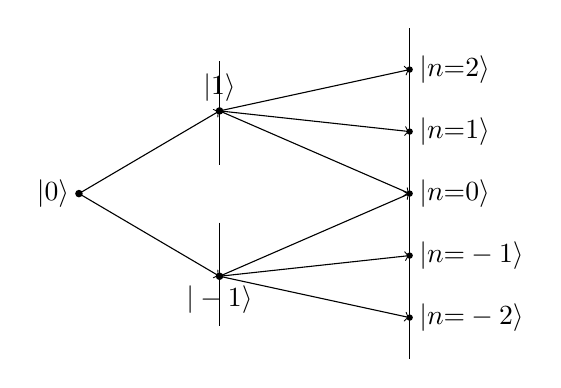
\begin{tikzpicture}[scale=1.05]
\fill (0,0) circle (1.3pt);
\node[left] at (0,0) {$|0\rangle$};

\draw (1.7,1.6) -- (1.7,0.35);
\draw (1.7,-0.35) -- (1.7,-1.6);
\fill (1.7,1) circle (1.3pt);
\fill (1.7,-1) circle (1.3pt);
\node[above] at (1.7,1) {$|1\rangle$};
\node[below] at (1.7,-1) {$|-1\rangle$};

\draw (4,2) -- (4,-2);
\fill (4,1.5) circle (1.1pt);
\fill (4,0.75) circle (1.1pt);
\fill (4,0) circle (1.1pt);
\fill (4,-0.75) circle (1.1pt);
\fill (4,-1.5) circle (1.1pt);
\node[right] at (4,1.5) {$|n{=}2\rangle$};
\node[right] at (4,0.75) {$|n{=}1\rangle$};
\node[right] at (4,0) {$|n{=}0\rangle$};
\node[right] at (4,-0.75) {$|n{=}-1\rangle$};
\node[right] at (4,-1.5) {$|n{=}-2\rangle$};

\draw[->] (0,0) -- (1.7,1);
\draw[->] (0,0) -- (1.7,-1);
\draw[->] (1.7,1) -- (4,1.5);
\draw[->] (1.7,1) -- (4,0.75);
\draw[->] (1.7,1) -- (4,0);
\draw[->] (1.7,-1) -- (4,0);
\draw[->] (1.7,-1) -- (4,-0.75);
\draw[->] (1.7,-1) -- (4,-1.5);
\end{tikzpicture}
\caption{A finite-state version of the two-slit experiment: source state \(|0\rangle\), two slit states \(|1\rangle\) and \(|-1\rangle\), and a screen basis \(|n\rangle\).}
\end{figure}

Now let the upper slit state evolve to a superposition on the screen,
\begin{equation}
|1\rangle \longrightarrow \sum_n \psi_n |n\rangle,
\end{equation}
and the lower slit state to another,
\begin{equation}
|-1\rangle \longrightarrow \sum_n \phi_n |n\rangle.
\end{equation}
By linearity,
\begin{equation}
|1\rangle+|-1\rangle \longrightarrow \sum_n (\psi_n+\phi_n)|n\rangle.
\end{equation}
So the amplitude at the screen site \(m\) is \(\psi_m+\phi_m\), and therefore
\begin{align}
P_m &= |\psi_m+\phi_m|^2 \\
    &= |\psi_m|^2+|\phi_m|^2+\psi_m^*\phi_m+\phi_m^*\psi_m.
\end{align}
The first two terms are what classical reasoning would have suggested: probability through the upper slit plus probability through the lower slit. The last two are interference.

At the symmetric point on the screen, call it \(m=0\), symmetry suggests \(\psi_0=\phi_0\). Then
\begin{equation}
P_0 = |\psi_0+\phi_0|^2 = |2\psi_0|^2 = 4|\psi_0|^2.
\end{equation}
Opening both slits gives four times the one-slit probability at that point, not twice. That is constructive interference.

A relative sign change can reverse the effect. If a phase shifter changes the lower amplitude so that \(\phi_0=-\psi_0\), then
\begin{equation}
P_0 = |\psi_0-\psi_0|^2 = 0.
\end{equation}
Each slit by itself allows arrival at that point, but opening both together can make arrival impossible. This is destructive interference.

One electron, of course, produces only one hit. The interference pattern is the accumulated probability distribution obtained from many repetitions of the same experiment, one particle at a time.

Now comes the measurement apparatus. Susskind introduces only one extra two-state system, a spin which begins in the down state. If the electron goes through the upper slit, it flips the spin to up. If it goes through the lower slit, it does nothing. The initial composite state is \(|0,d\rangle\), and the first update rule is
\begin{equation}
|0,d\rangle \longrightarrow |1,u\rangle + |-1,d\rangle.
\end{equation}
Already the structure has changed. This is no longer a superposition of states of one system. It is an entangled state of two systems: electron position and apparatus spin.

\begin{figure}[htbp]
\centering
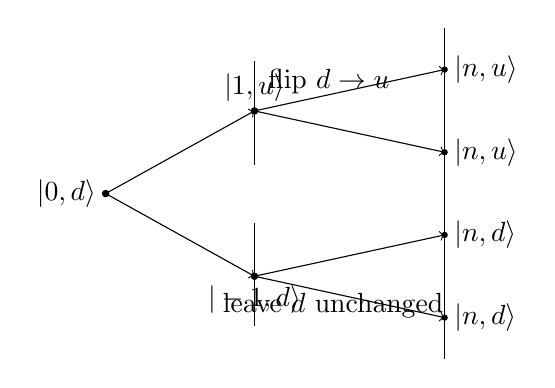
\begin{tikzpicture}[scale=1.05]
\fill (0,0) circle (1.3pt);
\node[left] at (0,0) {$|0,d\rangle$};

\draw (1.8,1.6) -- (1.8,0.35);
\draw (1.8,-0.35) -- (1.8,-1.6);
\fill (1.8,1) circle (1.3pt);
\fill (1.8,-1) circle (1.3pt);
\node[above] at (1.8,1) {$|1,u\rangle$};
\node[below] at (1.8,-1) {$|-1,d\rangle$};

\draw (4.1,2) -- (4.1,-2);
\fill (4.1,1.5) circle (1.1pt);
\fill (4.1,0.5) circle (1.1pt);
\fill (4.1,-0.5) circle (1.1pt);
\fill (4.1,-1.5) circle (1.1pt);
\node[right] at (4.1,1.5) {$|n,u\rangle$};
\node[right] at (4.1,0.5) {$|n,u\rangle$};
\node[right] at (4.1,-0.5) {$|n,d\rangle$};
\node[right] at (4.1,-1.5) {$|n,d\rangle$};

\draw[->] (0,0) -- (1.8,1);
\draw[->] (0,0) -- (1.8,-1);
\draw[->] (1.8,1) -- (4.1,1.5);
\draw[->] (1.8,1) -- (4.1,0.5);
\draw[->] (1.8,-1) -- (4.1,-0.5);
\draw[->] (1.8,-1) -- (4.1,-1.5);

\node at (2.7,1.35) {flip \(d\to u\)};
\node at (2.75,-1.35) {leave \(d\) unchanged};
\end{tikzpicture}
\caption{Measurement as entanglement with a detector spin. The upper path flips the apparatus spin; the lower path leaves it untouched.}
\end{figure}

Assume that after passing the slits the spin simply keeps its value while the electron continues to the screen:
\begin{align}
|1,u\rangle &\longrightarrow \sum_n \psi_n |n,u\rangle, \\
|-1,d\rangle &\longrightarrow \sum_n \phi_n |n,d\rangle.
\end{align}
Therefore, with both slits open,
\begin{equation}
|\Psi_{\mathrm{final}}\rangle
  = \sum_n \psi_n |n,u\rangle + \sum_n \phi_n |n,d\rangle.
\end{equation}

Now we compute the probability of arrival at site \(m\). The amplitude at that site is no longer a single complex number; it is the apparatus-spin state
\begin{equation}
\psi_m |u\rangle + \phi_m |d\rangle.
\end{equation}
Its norm squared is
\begin{align}
P_m
  &= \bigl(\psi_m^*\langle u|+\phi_m^*\langle d|\bigr)
     \bigl(\psi_m|u\rangle+\phi_m|d\rangle\bigr) \\
  &= |\psi_m|^2 + |\phi_m|^2
     + \psi_m^*\phi_m \langle u|d\rangle
     + \phi_m^*\psi_m \langle d|u\rangle.
\end{align}
But the record states are orthogonal:
\begin{equation}
\langle u|d\rangle=0.
\end{equation}
So the cross terms vanish, and we are left with
\begin{equation}
P_m = |\psi_m|^2 + |\phi_m|^2.
\end{equation}
That is the lecture's central result. Once which-path information is recorded, the amplitudes no longer interfere. Probabilities add the way they do in classical physics.

\subsection{Question \& Answer: What is the difference between a one-system superposition and a two-system entangled state?}

A state such as
\begin{equation}
|1\rangle+|-1\rangle
\end{equation}
is a superposition of states of one system. There is only the electron, and it is in a linear combination of two position states.

A state such as
\begin{equation}
|1,u\rangle+|-1,d\rangle
\end{equation}
is different in kind. Now there are two systems, electron and apparatus spin, and the state is not a statement about either one alone. It correlates them. By examining the spin one learns something about the electron's path. That is precisely why Susskind says that a measurement is the establishment of entanglement between the system and the apparatus.

The lecture closes by widening that point. A deliberately built detector is not the only possible recorder. An atom near the slit, a bit of gas, a thermal environment, any additional degree of freedom that becomes sufficiently entangled with the electron can destroy the interference pattern. If the environmental record states are fully distinguishable, the interference is fully destroyed. If they overlap only partially, the interference is only partially destroyed. Susskind stops there and leaves the quantitative treatment of weaker measurements for the next stage.

\section{Summary}

The lecture's mathematical spine is now visible. A property is represented not, in general, by a single state but by a subspace. The projector onto that subspace is built from an orthonormal basis of it, and the probability of the property is the expectation value of that projector. Compatible properties are combined, in the lecture's language, by multiplying commuting projectors. The same machinery then reappears in the two-slit problem: without a record, amplitudes add and interference appears; with a record, the electron becomes entangled with an apparatus, orthogonal record states kill the cross terms, and probabilities add instead. That is the lecture's version of collapse: not an extra postulate floating above the formalism, but the disappearance of interference when information about the alternatives has been deposited somewhere in the world.